\section{Exercise 8}
Cho mạch sau với \(p_2\), \(p_3\), \(p_4\) đang tiêu thụ công suất của các phần tử điện chưa biết. Đầu tiên, áp dụng kiến thức đã học để xác định chúng là phần tử active hay passive (cung cấp hay tiêu thụ công suất). Với một phần tử tiêu thụ công suất, dùng ký hiệu điện trở thuần với giá trị phù hợp làm phần tử đại diện. Với một phần tử cung cấp công suất, dùng ký hiệu của một nguồn điện một chiều lý tưởng với giá trị tương ứng làm phần tử đại diện. Kế tiếp, hãy vẽ lại mạch và tính toán công suất mà mỗi phần tử tiêu thụ. Lưu ý rằng chúng ta dùng quy ước dấu thụ động (passive sign convention). Sau đó, thực hiện mô phỏng với các phần tử đã được xác định.  

\begin{figure}[!htbp]
    \centering
    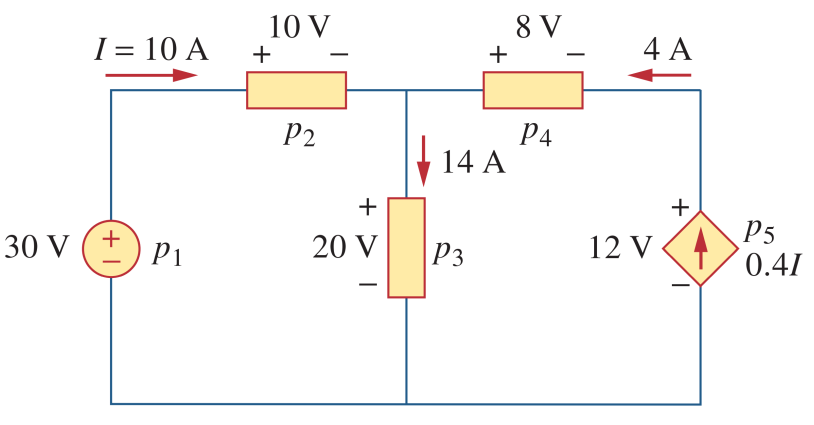
\includegraphics[width=0.7\textwidth]{graphics/ex8/f1.png}
    \caption{Mạch ban đầu}
\end{figure}


\subsection{Tính toán}

\begin{itemize}
    \item \(p_2 = I \cdot V = 10A \cdot 10V = 100W > 0\longrightarrow \) Đây là phần tử tiêu thụ công suất (passive).
    \item \(p_3 = I \cdot V = 14A \cdot 20V = 280W > 0\longrightarrow \) Đây là phần tử tiêu thụ công suất (passive).
    \item \(p_4 = I \cdot V = -4A \cdot 8V = -32W  < 0\longrightarrow \)  Đây là phần tử cung cấp công suất (active).
\end{itemize}

\subsection{Vẽ lại mạch và mô phỏng}
\begin{itemize}
    \item Đặt \(R_1 = p_2\) và \(R_2 = p_3\). Ta có: 

\(R_1 = \frac{U}{I} = \frac{10V}{10A} = 1\Omega\)

\(R_2 = \frac{U}{I} = \frac{20V}{14A} \approx 1.42857\Omega\)
\newpage

    \item Từ đó, ta có mạch mới như sau: 
\begin{figure}[!htbp]
    \centering
    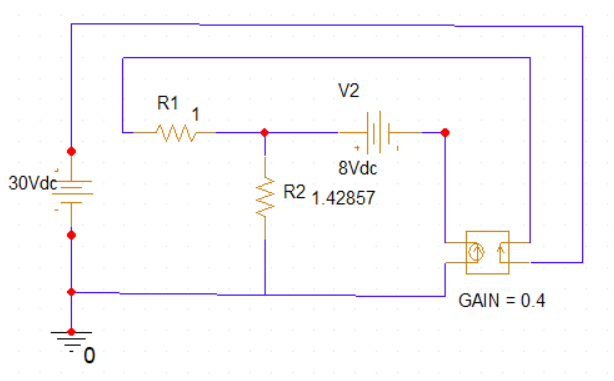
\includegraphics[width=0.7\textwidth]{graphics/ex8/f2.png}
    \caption{Mạch sau khi vẽ lại}
\end{figure}

    \item  Kết quả mô phỏng:
\begin{figure}[!htbp]
    \centering
    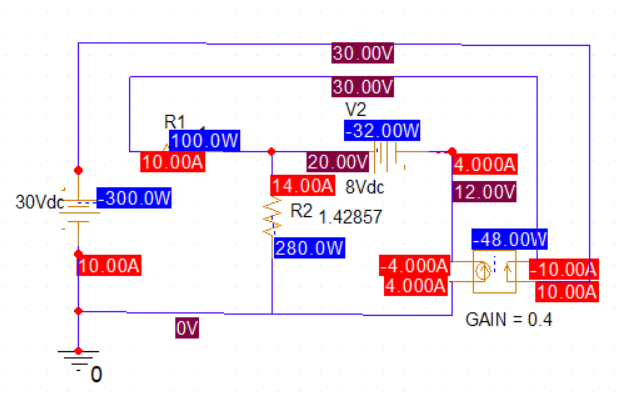
\includegraphics[width=0.7\textwidth]{graphics/ex8/f3.png}
    \caption{Mô phỏng}
\end{figure}

\end{itemize}